% !TEX root = ../main.tex
% 本文件由 build-tex.sh 从 31-DSP指南-第31章中译.md 生成，改内容请改 md 后重新生成

\chapter{复数傅里叶变换}\label{ch-31}

虽然复数从根本上和我们的现实世界脱节，但它可以用两种方式解决科学和工程问题。第一种，把真实世界问题中的参数代入成复数形式，这是上一章介绍的做法。第二种方式要优雅、强大得多：让复数在数学上与物理问题等价。这条路通向复数傅里叶变换(complex
Fourier transform)，它是第 8 章讨论的实数傅里叶变换(real Fourier
transform)的进阶版本。复数傅里叶变换本身很重要，同时也是通向更强大的复数技术（比如拉普拉斯变换和
z 变换）的垫脚石。这些复数变换是理论 DSP 的基础。

\section{实数 DFT}

傅里叶变换家族的四个成员（DFT、DTFT、傅里叶变换和傅里叶级数）都既可以用实数实现，也可以用复数实现。由于
DSP 主要关心 DFT，我们就拿它当例子。在跳进复数数学之前，先回顾一下实数
DFT，重点看看它在数学上有哪些别扭的地方。第 8
章按下面的公式定义了离散傅里叶变换的实数版本：

\textbf{公式 31-1}　实数
DFT。这是正变换，由时域算出频域。虽然用了''实部''和''虚部''这两个名字，这些公式里只有普通的数。频率下标
k 从 0 到 N/2。它们和公式 8-4 相同，只是把 2/N 这一项放进了正变换里。

\[\operatorname{Re}X[k] = \frac{2}{N}\sum_{n=0}^{N-1} x[n]\cos(2\pi kn/N)\]

\[\operatorname{Im}X[k] = \frac{-2}{N}\sum_{n=0}^{N-1} x[n]\sin(2\pi kn/N)\]

用文字说，一个 N 点的时域信号 x{[}n{]} 被分解成 N/2+1 个余弦波和 N/2+1
个正弦波，它们的频率由下标 k 给出。余弦波的幅度存放在 Re X{[}k{]}
中，正弦波的幅度存放在 Im X{[}k{]}
中。这些公式的做法是把相应的余弦波或正弦波与时域信号做相关。虽然用了''实部''和''虚部''这两个名字，这些公式里却没有任何复数，连一个
j 都看不到！我们还把归一化因子 2/N
放进了这些公式。记住，这个因子可以放在合成公式或分析公式的前面，也可以作为单独一步来处理（如公式
8-3
所述）。这些公式你应该在前面的章节里已经很熟悉了。如果还不熟，先回去复习这些概念再往下读。不懂实数
DFT，就永远不可能懂复数 DFT。

尽管实数 DFT
只用实数，借助代换(substitution)，频域还是可以用复数来表示。正如数组名所暗示的，Re
X{[}k{]} 成为复数频谱的实部，Im X{[}k{]}
成为虚部。换句话说，我们给虚部的每个值乘上一个
j，再和实部相加。但是，千万别误以为这就是''复数
DFT''。这只不过是做了复数代换的实数 DFT 而已。

实数 DFT
虽然足以应付科学和工程中的许多应用，但在数学上有三个别扭之处。第一，它只能通过代换来利用复数。这让数学家很不舒服，他们想说的是''这个等于那个''，而不只是''这个代表那个''。举个例子，假设给你一个数学命题：A
等于
B。我们立刻就知道无数推论：\(5A = 5B\)，\(1+A = 1+B\)，\(A/x = B/x\)，等等。再假设给你的命题是：A
代表
B。没有更多信息的话，我们什么都不知道！当两样东西相等时，我们可以动用四千年积累的数学；当它们只是互相代表时，就得用新的定义从头开始。例如，用复数表示正弦信号时，我们允许做加减，却禁止做乘除。

实数傅里叶变换处理得不好的第二件事，是频谱的负频率(negative
frequency)部分。回忆第 10
章，正弦波和余弦波既可以描述成正频率，也可以描述成负频率。由于这两种看法完全等价，实数傅里叶变换就把负频率忽略了。然而，有些应用中负频率很重要。当负频率成分被迫移到频谱的正频率部分时，就会出现这种情况。可以说，鬼魂现出了人形。例如，混叠、循环卷积和幅度调制中发生的就是这种事。由于实数傅里叶变换不用负频率，它应付这些情况的能力非常有限。

我们的第三个不满，是 Re X{[}0{]} 和 Re X{[}N/2{]}
这两点（频谱的第一个和最后一个点）需要特殊处理。假设我们从一个 N 点信号
x{[}n{]} 出发，做 DFT 得到存放在 Re X{[}k{]} 和 Im X{[}k{]} 中的频谱，k
从 0 到 N/2。但这些并不是重建时域波形所需的幅度：Re X{[}0{]} 和 Re
X{[}N/2{]} 两个采样必须先除以二。（可以回看公式 8-3
温习一下。）这在程序里很容易做到，但在公式里处理起来很不方便。

复数傅里叶变换是解决这些问题的优雅方案。复数和负频率天生就是相伴而行的。我们来看看它是怎么做到的。

\section{数学上的等价}

第一步，说明怎样把正弦波和余弦波写成含复数的等式。关键是上一章介绍的欧拉关系(Euler's
relation)：

\textbf{公式 31-2}　欧拉关系。

\[e^{jx} = \cos(x) + j\sin(x)\]

乍一看，这似乎没多大用处：一个复数表达式等于另一个复数表达式。不过，稍做一点代数，就能把这个关系改写成另外两种形式：

\textbf{公式 31-3}　正弦和余弦的欧拉关系。

\[\cos(x) = \frac{e^{jx} + e^{-jx}}{2} \qquad\qquad \sin(x) = \frac{e^{jx} - e^{-jx}}{2j}\]

这个结果极其重要：我们找到了一种在复数和普通正弦信号之间写等式的方法。公式
31-3
虽然是这个恒等式的标准形式，但为了这里的讨论，把几项调换一下会更有用：

\textbf{公式
31-4}　用复数表示正弦信号。借助复数，余弦波和正弦波都可以写成一个正频率与一个负频率之和。

\[\cos(\omega t) = \tfrac{1}{2}\,e^{j(-\omega)t} + \tfrac{1}{2}\,e^{j\omega t}\]

\[\sin(\omega t) = \tfrac{1}{2}\,j\,e^{j(-\omega)t} - \tfrac{1}{2}\,j\,e^{j\omega t}\]

每个表达式都是两个指数之和：一个含正频率（ω），另一个含负频率（−ω）。换句话说，把正弦波和余弦波写成复数时，频谱的负频率部分就自动包含进来了。正频率和负频率地位平等，各需要一半才能组成一个完整的波形。

\section{复数 DFT}

复数 DFT 的正变换写成极坐标形式(polar form)是：

\textbf{公式 31-5}　复数 DFT 正变换。时域 x{[}n{]} 和频域 X{[}k{]}
都是复数数组，k 和 n 都从 0 到 N−1。这个公式是极坐标形式，也是 DSP
中最常用的形式。

\[X[k] = \frac{1}{N}\sum_{n=0}^{N-1} x[n]\,e^{-j2\pi kn/N}\]

也可以用欧拉关系把正变换改写成直角坐标形式(rectangular form)：

\textbf{公式 31-6}　复数 DFT 正变换（直角坐标形式）。

\[X[k] = \frac{1}{N}\sum_{n=0}^{N-1} x[n]\,\big[\cos(2\pi kn/N) - j\sin(2\pi kn/N)\big]\]

先拿这个复数傅里叶变换的公式和实数傅里叶变换的公式 31-1
比较一下。乍一看两者好像一样，只需一点点代数就能把公式 31-6 变成公式
31-1。然而这很有误导性：两个公式之间的区别非常细微、很容易忽略，却极其重要。我们逐条细看这些区别。

第一，实数傅里叶变换把一个实数时域信号 x{[}n{]} 变成两个实数频域信号 Re
X{[}k{]} 和 Im X{[}k{]}。借助复数代换，频域可以用一个复数数组 X{[}k{]}
来表示。而在复数傅里叶变换中，x{[}n{]} 和 X{[}k{]}
都是复数数组。一个实用的提示：时域虽然是复数，但没有任何规定要求我们必须用到虚部。假设我们要处理一个实信号，比如随时间采集的一串电压测量值。这组数据就作为时域信号的实部，虚部则全为零。

第二，实数傅里叶变换只处理正频率，也就是说，频域下标 k 只从 0 走到
N/2。相比之下，复数傅里叶变换同时包含正频率和负频率，这意味着 k 从 0
走到 N−1。0 到 N/2 之间的频率是正的，N/2 到 N−1
之间的频率是负的。记住，离散信号的频谱是周期性的，所以 N/2 到 N−1
之间的负频率与 −N/2 到 0 之间的负频率是一回事。0 和 N/2
这两个采样骑在正负频率的分界线上。如果需要温习，可以回看第 10 章和第 12
章。

第三，在做了代换的实数傅里叶变换中，正弦波各项被加上了一个
j，使频谱能用复数表示。要变回普通的正弦和余弦波，直接把 j
去掉就行。这就是''一样东西只是代表另一样东西''时带来的随意性。相比之下，复数
DFT（公式 31-5）是一个正式的数学等式，j
是其中不可分割的一部分。从这个角度看，我们不能随意添上或去掉一个
j，就像不能随意添上或去掉等式中的其他变量一样。

第四，实数傅里叶变换前面有一个因子
2，而复数傅里叶变换没有。假设我们对一个幅度为一的余弦波做实数
DFT，对应这个余弦波的频谱值也是一。现在改用复数 DFT
重复这个过程。这时余弦波对应两个频谱值，一个正频率、一个负频率，两者的值都是
½。换句话说，幅度为 ½ 的正频率与幅度为 ½
的负频率合在一起，产生一个幅度为一的余弦波。

第五，实数傅里叶变换需要对两个频域采样 Re X{[}0{]} 和 Re X{[}N/2{]}
做特殊处理，而复数傅里叶变换不需要。假设我们从一个时域信号出发，做 DFT
求出频域信号。要反过来，就对频域信号做逆
DFT，重建原来的时域信号。不过，要让重建的信号与原信号完全相同，需要做缩放。对复数傅里叶变换来说，必须在某个环节引入一个
1/N
因子。它可以挂在正变换上、挂在逆变换上，或者在两者之间单独作为一步。对实数傅里叶变换来说，还需要再乘一个因子二（即
2/N），如上所述。此外，实数傅里叶变换还需要一个额外的缩放步骤：Re
X{[}0{]} 和 Re X{[}N/2{]}
必须在某个环节除以二。换句话说，这两个采样用的缩放因子是
1/N，而频谱其余部分用的是
2/N。前面说过，这个别扭的步骤正是我们对实数傅里叶变换的不满之一。

为什么实数 DFT 和复数 DFT
对这两点的处理不同？要回答这个问题，记住：时域中的一个余弦（或正弦）波，在复数
DFT
的频谱中会一分为二，分到一个正频率和一个负频率上。但有两个例外，就是位于
0 和 N/2
的频谱值。它们对应零频率（直流）和奈奎斯特频率（采样率的一半）。由于这两点骑在频谱正负两部分的分界线上，它们没有与之配对的点。因为不与另一个值合并，它们对时域的贡献天生就只有其他频率的一半。

\begin{figure}[htbp]
\centering
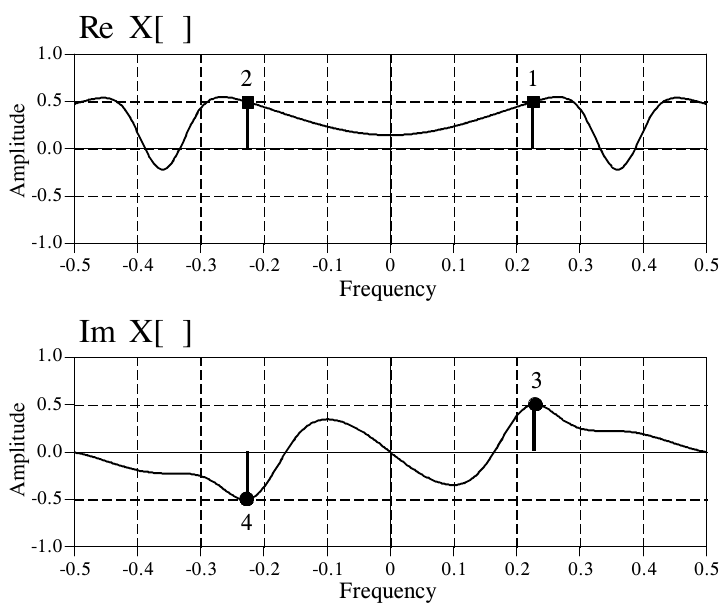
\includegraphics[width=0.604\linewidth,height=0.8\textheight,keepaspectratio]{assets/ch31/fig31-01.png}
\caption*{\textbf{图 31-1　复数频谱。}
这两条曲线对应一个纯实数的时域信号，因为频谱的实部具有偶对称性，虚部具有奇对称性。实部中的两个方形标记对应一个幅度为一、频率为
0.23 的余弦波。虚部中的两个圆形标记对应一个幅度为一、频率为 0.23
的正弦波。 （Re X{[} {]} = 实部，Im X{[} {]} = 虚部；Amplitude =
幅度，Frequency = 频率。图中数字 1～4 是正文引用的标号：1、2 是实部在
±0.23 处的方形标记，3、4 是虚部在 ±0.23 处的圆形标记。）}
\end{figure}

图 31-1 展示了复数 DFT
的频谱。这张图假设时域完全是实数，也就是说它的虚部为零。虚数时域信号的概念稍后再讨论。显示复数频谱有两种常见方式。如图所示，可以把零频率放在中间，正频率在右、负频率在左。这是思考完整频谱的最好方式，也是显示非周期频谱的唯一方式。

问题在于，离散信号的频谱是周期性的（比如 DFT 和 DTFT）。这意味着 −0.5 到
0.5 之间的一切会向左、向右无限次重复。这种情况下，0 到 1.0 之间的频谱与
−0.5 到 0.5 之间包含的信息完全相同。画图时，比如图 31-1，通常采用 −0.5
到 0.5 的约定。然而，许多公式和程序采用 0 到 1.0 的形式。例如，在公式
31-5 和 31-6 中，频率下标 k 从 0 走到 N−1（对应 0 到
1.0）。不过，只要愿意，也可以把它写成从 −N/2 走到 N/2−1（对应 −0.5 到
0.5）。

以图 31-1 的频谱为例，可以考察逆复数 DFT 怎样重建时域信号。逆复数 DFT
写成极坐标形式是：

\textbf{公式 31-7}　逆复数 DFT。它是与公式 31-5 的复数 DFT
正变换相配对的公式。

\[x[n] = \sum_{k=0}^{N-1} X[k]\,e^{j2\pi kn/N}\]

用欧拉关系，可以把它写成直角坐标形式：

\textbf{公式 31-8}　逆复数 DFT。这是把公式 31-7
改写后的形式，展示频谱中每个值怎样影响时域。

\[x[n] = \sum_{k=0}^{N-1} \operatorname{Re}X[k]\,\big[\cos(2\pi kn/N) + j\sin(2\pi kn/N)\big] \;-\; \sum_{k=0}^{N-1} \operatorname{Im}X[k]\,\big[\sin(2\pi kn/N) - j\cos(2\pi kn/N)\big]\]

逆 DFT 通常写成公式 31-7 的紧凑形式，不过公式 31-8
的展开形式可能更容易理解。

\begin{quote}
\textbf{译注：} 原文此处写的是''the expanded version in Eq.
31-9''，但本章没有公式 31-9，指的应是刚给出的公式 31-8。
\end{quote}

用文字说，频域实部中的每个值，都向时域贡献一个实余弦波和一个虚正弦波。同样，频域虚部中的每个值，都向时域贡献一个实正弦波和一个虚余弦波。把所有这些实的和虚的正弦信号加起来，就得到时域。重要的概念是：频域中的每个值，都在时域中同时产生一个实正弦信号和一个虚正弦信号。

例如，设想我们要重建一个频率为
2πk/N、幅度为一的余弦波。这需要一个正频率和一个负频率，两者都来自频谱的实部。图
31-1 中的两个方形标记就是一个例子，频率设为 k/N = 0.23。位于 0.23
的正频率（图 31-1 中标为 1）向时域贡献一个余弦波和一个虚正弦波：

\[\tfrac{1}{2}\cos(2\pi\,0.23\,n) + \tfrac{1}{2}\,j\sin(2\pi\,0.23\,n)\]

同样，位于 −0.23 的负频率（图 31-1 中标为
2）也向时域贡献一个余弦波和一个虚正弦波：

\[\tfrac{1}{2}\cos(2\pi(-0.23)n) + \tfrac{1}{2}\,j\sin(2\pi(-0.23)n)\]

利用关系式 \(\cos(-x) = \cos(x)\) 和
\(\sin(-x) = -\sin(x)\)，可以去掉余弦和正弦项里的负号。于是负频率的贡献可以改写成：

\[\tfrac{1}{2}\cos(2\pi\,0.23\,n) - \tfrac{1}{2}\,j\sin(2\pi\,0.23\,n)\]

把正频率和负频率的贡献加起来，就重建出了时域信号：

{\def\LTcaptype{none} % do not increment counter
\begin{longtable}[]{@{}
  >{\raggedright\arraybackslash}p{(\linewidth - 2\tabcolsep) * \real{0.5000}}
  >{\raggedright\arraybackslash}p{(\linewidth - 2\tabcolsep) * \real{0.5000}}@{}}
\toprule\noalign{}
\endhead
\bottomrule\noalign{}
\endlastfoot
正频率的贡献 \dspsym{→} &
\(\tfrac{1}{2}\cos(2\pi\,0.23\,n) + \tfrac{1}{2}\,j\sin(2\pi\,0.23\,n)\) \\
负频率的贡献 \dspsym{→} &
\(\tfrac{1}{2}\cos(2\pi\,0.23\,n) - \tfrac{1}{2}\,j\sin(2\pi\,0.23\,n)\) \\
得到的时域信号 \dspsym{→} & \(\cos(2\pi\,0.23\,n)\) \\
\end{longtable}
}

用同样的方法，可以在时域合成一个正弦波。这时需要来自频谱虚部的一个正频率和一个负频率，也就是图
31-1 中的圆形标记。按公式
31-8，这些频谱值向时域贡献一个正弦波和一个虚余弦波。虚余弦波互相抵消，而实正弦波相加：

{\def\LTcaptype{none} % do not increment counter
\begin{longtable}[]{@{}
  >{\raggedright\arraybackslash}p{(\linewidth - 2\tabcolsep) * \real{0.5000}}
  >{\raggedright\arraybackslash}p{(\linewidth - 2\tabcolsep) * \real{0.5000}}@{}}
\toprule\noalign{}
\endhead
\bottomrule\noalign{}
\endlastfoot
正频率的贡献 \dspsym{→} &
\(-\tfrac{1}{2}\sin(2\pi\,0.23\,n) + \tfrac{1}{2}\,j\cos(2\pi\,0.23\,n)\) \\
负频率的贡献 \dspsym{→} &
\(-\tfrac{1}{2}\sin(2\pi\,0.23\,n) - \tfrac{1}{2}\,j\cos(2\pi\,0.23\,n)\) \\
得到的时域信号 \dspsym{→} & \(-\sin(2\pi\,0.23\,n)\) \\
\end{longtable}
}

\begin{quote}
\textbf{译注：} 原书这两行虚余弦项的正负号印反了：正频率一行印作
\(-\tfrac{1}{2}j\cos\)，负频率一行印作 \(+\tfrac{1}{2}j\cos\)。按公式
31-8 代入（正频率处 Im X = +0.5，负频率处 Im X = −0.5），正频率贡献的是
\(+\tfrac{1}{2}j\cos\)，负频率是
\(-\tfrac{1}{2}j\cos\)，上表已改正。两行相加的结果（\(-\sin\)）不受影响。我用
Python 代入 n = 3 数值核对过。
\end{quote}

注意，虽然正频率的值是正的，生成的却是一个负的正弦波。这个符号反转是复数
DFT 数学固有的一部分。你可能还记得，实数 DFT
中也常用同样的符号反转，也就是说，频谱虚部中的正值对应一个负的正弦波。大多数作者把这个符号反转写进实数傅里叶变换的定义里，让它与复数版本保持一致。要点在于：复数傅里叶变换必须使用这个符号反转，而在实数傅里叶变换中它只是一个可选项。

复数傅里叶变换的对称性非常重要。如图 31-1
所示，实数时域信号对应的频谱，实部是偶对称的，虚部是奇对称的。换句话说，在实部中，负频率和正频率同号（比如图
31-1 中的点 1 和点 2）；而在虚部中，它们异号（点 3 和点 4）。

这又引出了另一个话题：时域的虚部。到目前为止，我们一直假设时域完全是实数，也就是虚部为零。然而，复数傅里叶变换并不要求这一点。虚数时域信号有什么物理意义？通常没有。这只是复数数学允许的东西，在我们生活的世界里没有对应物。不过，在某些应用中，可以出于数学目的利用或操纵它。

第 12
章就给出了一个例子。时域的虚部产生的频谱，实部是奇对称的，虚部是偶对称的。这恰好和时域实部产生的频谱（图
31-1）相反。当时域同时含有实部和虚部时，频谱等于两者分别计算所得频谱之和。第
12 章介绍了怎样利用这一点，让 FFT
算法一次算出两个实信号的频谱：一个信号放进时域的实部，另一个放进虚部。FFT
计算完成后，再用奇偶分解把两个信号的频谱分开。

\section{傅里叶变换家族}

正如 DFT
有实数和复数两个版本，傅里叶变换家族的其他成员也一样。这就产生了表 31-1
中的一大堆公式。不要逐个去背这些公式，而要把它们当作一个组织良好、对称的整体来理解。下面的说明描述了傅里叶变换家族的组织方式。内容详细、重复，而且枯燥。尽管如此，这是理解理论
DSP 所需的背景知识。好好学。

\textbf{1. 四种傅里叶变换}

时域信号可以是连续的或离散的，也可以是周期的或非周期的。由此定义了四种傅里叶变换：离散傅里叶变换（Discrete
Fourier Transform，离散、周期）、离散时间傅里叶变换（Discrete Time
Fourier Transform，离散、非周期）、傅里叶级数（Fourier
Series，连续、周期）和傅里叶变换（Fourier
Transform，连续、非周期）。别去琢磨这些名字背后的道理，根本没有道理可言。

如果信号在一个域中是离散的，它在另一个域中就是周期的。同样，如果信号在一个域中是连续的，它在另一个域中就是非周期的。连续信号用圆括号
( ) 表示，离散信号用方括号 {[} {]}
表示。没有记号用来表示信号是周期的还是非周期的。

\textbf{2. 实数与复数}

这四种变换各有一个复数版本和一个实数版本。复数版本的时域信号和频域信号都是复数。实数版本有一个实数时域信号和两个实数频域信号。复数情形同时使用正频率和负频率，而实数变换只使用正频率。复数变换通常写成指数形式，不过如有需要，可以用欧拉关系把它们改写成余弦和正弦形式。

\textbf{3. 分析与合成}

每种变换都有一个分析公式（analysis
equation，也叫正变换）和一个合成公式（synthesis
equation，也叫逆变换）。分析公式说明怎样根据时域中的所有值，算出频域中的每个值。合成公式说明怎样根据频域中的所有值，算出时域中的每个值。

\textbf{4. 时域记号}

连续时域信号记作 x(t)，离散时域信号记作
x{[}n{]}。对复数变换，这些信号是复数；对实数变换，这些信号是实数。所有时域信号都从负无穷延伸到正无穷。不过，如果时域是周期性的，我们只关心一个周期，因为其余部分都是重复的。变量
T 和 N 分别表示连续信号和离散信号在时域中的周期。

\textbf{5. 频域记号}

连续频域信号如果是复数，记作 X(ω)；如果是实数，记作 Re X(ω) 和 Im
X(ω)。离散频域信号如果是复数，记作 X{[}k{]}；如果是实数，记作 Re
X{[}k{]} 和 Im
X{[}k{]}。复数变换的负频率从负无穷延伸到零，正频率从零延伸到正无穷。实数变换只使用正频率。如果频域是周期性的，我们只关心一个周期，因为其余部分都是重复的。对于连续频域，自变量
ω 从 −π 到 π 走完一个完整周期。在离散情形中，我们使用 k 从 0 到 N−1
的那个周期。

\begin{quote}
\textbf{译注：} 这里说连续频域的一个周期取 −π 到 π，但表 31-1 中 DTFT
复数形式的合成公式积分区间写的是 0 到
2π。两者都是一个完整周期，结果相同（见下面第 6、7 条）。
\end{quote}

\textbf{6. 分析公式}

分析公式通过相关来运作，即把时域信号乘以一个正弦信号，再在合适的时域区间上积分（连续时域）或求和（离散时域）。如果时域信号是非周期的，合适的区间是从负无穷到正无穷。如果时域信号是周期的，合适的区间是任意一个完整周期。这里给出的公式都是在
0 到 T（或 0 到
N−1）这个周期上积分（或求和）的。不过，换成其他任何一个完整周期，结果都完全相同，比如
−T 到 0、−T/2 到 T/2 等等。

\textbf{7. 合成公式}

合成公式说明时域中的单个值怎样由频域中的所有点算出。做法是把频域乘以一个正弦信号，再在合适的频域区间上积分（连续频域）或求和（离散频域）。如果频域是复数且非周期的，合适的区间是负无穷到正无穷。如果频域是复数且周期的，合适的区间是一个完整周期，即
−π 到 π（连续频域）或 0 到
N−1（离散频域）。如果频域是实数且非周期的，合适的区间是零到正无穷，也就是只取正频率。最后，如果频域是实数且周期的，合适的区间是包含正频率的那半个周期，即
0 到 π（连续频域）或 0 到 N/2（离散频域）。

\textbf{8. 缩放}

要让分析公式和合成公式互为逆运算，必须在其中一个公式上放一个缩放因子。在表
31-1 中，我们把缩放因子放在了分析公式上。在复数情形中，这些缩放因子是
1/N、1/T 或 1/2π。由于实数变换不用负频率，它们的缩放因子大一倍：2/N、2/T
或
1/π。实数变换在计算频谱虚部时还多了一个负号（这是一个可选项，用来让实数变换与复数变换更一致）。最后，实数
DFT 和实数傅里叶级数的合成公式对 Re X(0) 和 Re X{[}N/2{]}
有特殊的缩放说明。

\textbf{9. 变体}

这些公式在其他出版物中可能长得不一样。下面是几种需要留意的变体：

\begin{itemize}
\tightlist
\item
  用 f 代替 ω，关系为 \(\omega = 2\pi f\)
\item
  在其他周期上积分，比如 −T 到 0、−T/2 到 T/2，或 0 到 T
\item
  把全部或部分缩放因子移到合成公式上
\item
  用基频 \(f_0 = 1/T\) 代替周期
\item
  使用其他变量名，例如在 DTFT 中 ω 可能写成 Ω，傅里叶级数中的 Re
  X{[}k{]} 和 Im X{[}k{]} 可能写成 \(a_k\) 和 \(b_k\)
\end{itemize}

\subsection{表 31-1　傅里叶变换}

\textbf{离散傅里叶变换（DFT）}

{\def\LTcaptype{none} % do not increment counter
\begin{longtable}[]{@{}
  >{\raggedright\arraybackslash}p{(\linewidth - 4\tabcolsep) * \real{0.3333}}
  >{\raggedright\arraybackslash}p{(\linewidth - 4\tabcolsep) * \real{0.3333}}
  >{\raggedright\arraybackslash}p{(\linewidth - 4\tabcolsep) * \real{0.3333}}@{}}
\toprule\noalign{}
\begin{minipage}[b]{\linewidth}\raggedright
\end{minipage} & \begin{minipage}[b]{\linewidth}\raggedright
复数变换
\end{minipage} & \begin{minipage}[b]{\linewidth}\raggedright
实数变换
\end{minipage} \\
\midrule\noalign{}
\endhead
\bottomrule\noalign{}
\endlastfoot
合成 & \(x[n] = \displaystyle\sum_{k=0}^{N-1} X[k]\,e^{j2\pi kn/N}\) &
\(x[n] = \displaystyle\sum_{k=0}^{N/2} \operatorname{Re}X[k]\cos(2\pi kn/N) - \operatorname{Im}X[k]\sin(2\pi kn/N)\) \\
分析 &
\(X[k] = \dfrac{1}{N}\displaystyle\sum_{n=0}^{N-1} x[n]\,e^{-j2\pi kn/N}\)
&
\(\operatorname{Re}X[k] = \dfrac{2}{N}\displaystyle\sum_{n=0}^{N-1} x[n]\cos(2\pi kn/N)\)；\(\operatorname{Im}X[k] = \dfrac{-2}{N}\displaystyle\sum_{n=0}^{N-1} x[n]\sin(2\pi kn/N)\) \\
时域 & x{[}n{]} 是复数、离散、周期的；n 在一个周期内从 0 到 N−1 &
x{[}n{]} 是实数、离散、周期的；n 在一个周期内从 0 到 N−1 \\
频域 & X{[}k{]} 是复数、离散、周期的；k 在一个周期内从 0 到 N−1；k = 0
到 N/2 是正频率，k = N/2 到 N−1 是负频率 & Re X{[}k{]}、Im X{[}k{]}
都是实数、离散、周期的；k 在半个周期内从 0 到 N/2 \\
注意 & & 使用合成公式之前，Re X{[}0{]} 和 Re X{[}N/2{]} 必须先除以二 \\
\end{longtable}
}

\textbf{离散时间傅里叶变换（DTFT）}

{\def\LTcaptype{none} % do not increment counter
\begin{longtable}[]{@{}
  >{\raggedright\arraybackslash}p{(\linewidth - 4\tabcolsep) * \real{0.3333}}
  >{\raggedright\arraybackslash}p{(\linewidth - 4\tabcolsep) * \real{0.3333}}
  >{\raggedright\arraybackslash}p{(\linewidth - 4\tabcolsep) * \real{0.3333}}@{}}
\toprule\noalign{}
\begin{minipage}[b]{\linewidth}\raggedright
\end{minipage} & \begin{minipage}[b]{\linewidth}\raggedright
复数变换
\end{minipage} & \begin{minipage}[b]{\linewidth}\raggedright
实数变换
\end{minipage} \\
\midrule\noalign{}
\endhead
\bottomrule\noalign{}
\endlastfoot
合成 &
\(x[n] = \displaystyle\int_{0}^{2\pi} X(\omega)\,e^{j\omega n}\,d\omega\)
&
\(x[n] = \displaystyle\int_{0}^{\pi} \operatorname{Re}X(\omega)\cos(\omega n) - \operatorname{Im}X(\omega)\sin(\omega n)\,d\omega\) \\
分析 &
\(X(\omega) = \dfrac{1}{2\pi}\displaystyle\sum_{n=-\infty}^{+\infty} x[n]\,e^{-j\omega n}\)
&
\(\operatorname{Re}X(\omega) = \dfrac{1}{\pi}\displaystyle\sum_{n=-\infty}^{+\infty} x[n]\cos(\omega n)\)；\(\operatorname{Im}X(\omega) = \dfrac{-1}{\pi}\displaystyle\sum_{n=-\infty}^{+\infty} x[n]\sin(\omega n)\) \\
时域 & x{[}n{]} 是复数、离散、非周期的；n 从负无穷到正无穷 & x{[}n{]}
是实数、离散、非周期的；n 从负无穷到正无穷 \\
频域 & X(ω) 是复数、连续、周期的；ω 在一个周期内从 0 到 2π；ω = 0 到 π
是正频率，ω = π 到 2π 是负频率 & Re X(ω)、Im X(ω)
都是实数、连续、周期的；ω 在半个周期内从 0 到 π \\
\end{longtable}
}

\textbf{傅里叶级数}

{\def\LTcaptype{none} % do not increment counter
\begin{longtable}[]{@{}
  >{\raggedright\arraybackslash}p{(\linewidth - 4\tabcolsep) * \real{0.3333}}
  >{\raggedright\arraybackslash}p{(\linewidth - 4\tabcolsep) * \real{0.3333}}
  >{\raggedright\arraybackslash}p{(\linewidth - 4\tabcolsep) * \real{0.3333}}@{}}
\toprule\noalign{}
\begin{minipage}[b]{\linewidth}\raggedright
\end{minipage} & \begin{minipage}[b]{\linewidth}\raggedright
复数变换
\end{minipage} & \begin{minipage}[b]{\linewidth}\raggedright
实数变换
\end{minipage} \\
\midrule\noalign{}
\endhead
\bottomrule\noalign{}
\endlastfoot
合成 &
\(x(t) = \displaystyle\sum_{k=-\infty}^{+\infty} X[k]\,e^{j2\pi kt/T}\)
&
\(x(t) = \displaystyle\sum_{k=0}^{+\infty} \operatorname{Re}X[k]\cos(2\pi kt/T) - \operatorname{Im}X[k]\sin(2\pi kt/T)\) \\
分析 &
\(X[k] = \dfrac{1}{T}\displaystyle\int_{0}^{T} x(t)\,e^{-j2\pi kt/T}\,dt\)
&
\(\operatorname{Re}X[k] = \dfrac{2}{T}\displaystyle\int_{0}^{T} x(t)\cos(2\pi kt/T)\,dt\)；\(\operatorname{Im}X[k] = \dfrac{-2}{T}\displaystyle\int_{0}^{T} x(t)\sin(2\pi kt/T)\,dt\) \\
时域 & x(t) 是复数、连续、周期的；t 在一个周期内从 0 到 T & x(t)
是实数、连续、周期的；t 在一个周期内从 0 到 T \\
频域 & X{[}k{]} 是复数、离散、非周期的；k 从负无穷到正无穷；k
\textgreater{} 0 是正频率，k \textless{} 0 是负频率 & Re X{[}k{]}、Im
X{[}k{]} 都是实数、离散、非周期的；k 从零到正无穷 \\
注意 & & 使用合成公式之前，Re X{[}0{]} 必须先除以二 \\
\end{longtable}
}

\textbf{傅里叶变换}

{\def\LTcaptype{none} % do not increment counter
\begin{longtable}[]{@{}
  >{\raggedright\arraybackslash}p{(\linewidth - 4\tabcolsep) * \real{0.3333}}
  >{\raggedright\arraybackslash}p{(\linewidth - 4\tabcolsep) * \real{0.3333}}
  >{\raggedright\arraybackslash}p{(\linewidth - 4\tabcolsep) * \real{0.3333}}@{}}
\toprule\noalign{}
\begin{minipage}[b]{\linewidth}\raggedright
\end{minipage} & \begin{minipage}[b]{\linewidth}\raggedright
复数变换
\end{minipage} & \begin{minipage}[b]{\linewidth}\raggedright
实数变换
\end{minipage} \\
\midrule\noalign{}
\endhead
\bottomrule\noalign{}
\endlastfoot
合成 &
\(x(t) = \displaystyle\int_{-\infty}^{+\infty} X(\omega)\,e^{j\omega t}\,d\omega\)
&
\(x(t) = \displaystyle\int_{0}^{+\infty} \operatorname{Re}X(\omega)\cos(\omega t) - \operatorname{Im}X(\omega)\sin(\omega t)\,d\omega\) \\
分析 &
\(X(\omega) = \dfrac{1}{2\pi}\displaystyle\int_{-\infty}^{+\infty} x(t)\,e^{-j\omega t}\,dt\)
&
\(\operatorname{Re}X(\omega) = \dfrac{1}{\pi}\displaystyle\int_{-\infty}^{+\infty} x(t)\cos(\omega t)\,dt\)；\(\operatorname{Im}X(\omega) = \dfrac{-1}{\pi}\displaystyle\int_{-\infty}^{+\infty} x(t)\sin(\omega t)\,dt\) \\
时域 & x(t) 是复数、连续、非周期的；t 从负无穷到正无穷 & x(t)
是实数、连续、非周期的；t 从负无穷到正无穷 \\
频域 & X(ω) 是复数、连续、非周期的；ω 从负无穷到正无穷；ω \textgreater{}
0 是正频率，ω \textless{} 0 是负频率 & Re X(ω)、Im X(ω)
都是实数、连续、非周期的；ω 从零到正无穷 \\
\end{longtable}
}

\begin{quote}
\textbf{译注：} 表 31-1 中有几处原书排印问题，上表已改正： -
傅里叶变换实数形式的合成公式，积分变量印成了 dt，应为 dω（被积函数是 ω
的函数）。 - 傅里叶变换实数形式的频域说明，把 Re X(ω)、Im X(ω)
印成了方括号 Re X{[}ω{]}、Im
X{[}ω{]}。按本表的记号约定，连续信号用圆括号。 -
傅里叶变换复数形式的说明里 continuous 两处拼成了 continious。
\end{quote}

\section{为什么要用复数傅里叶变换}

从本章可以痛苦地看出，复数 DFT 比实数 DFT 复杂得多。复数 DFT
带来的好处，真的值得花力气去学那些错综复杂的数学吗？这个问题的答案取决于你是谁，以及你打算拿
DSP 做什么。本书的一个基本前提是：大多数实用的 DSP
技术，不借助复数变换也能理解和使用。如果你学 DSP 是为了辅助你在 DSP
以外的研究或工程工作，复数 DFT 大概是杀鸡用牛刀。

尽管如此，复数数学是 DSP
专业人员的主要语言。如果你不懂这门语言，就没法和这个领域的专业人士交流，包括读懂
DSP 文献：书籍、论文、技术文章等等。为什么复数技术在 DSP
专业圈子里这么流行？我们已经提到了几个原因：公式紧凑；分析公式与合成公式之间的对称性；时域与频域之间的对称性；包含负频率；是通向拉普拉斯变换和
z 变换的垫脚石，等等。

还有一个更具哲学意味、我们还没讨论过的原因，那就是真理。本章一开始列举了实数傅里叶变换的几处别扭之处。引入复数傅里叶变换之后，这些问题都消失了。我们说：太好了，复数傅里叶变换解决了这些难题。

这话没错，但没有给复数傅里叶变换应有的评价。换个角度看这件事：尽管复数傅里叶变换很抽象，它却恰当地描述了物理系统的行为。当我们把数学限制在实数范围内时，问题就出现了。换句话说，这些问题不是被复数傅里叶变换解决的，而是被实数傅里叶变换引入的。在数学的世界里，复数傅里叶变换是比实数傅里叶变换更高的真理。这对数学家和学术界有着巨大的吸引力，这个群体致力于拓展人类的知识，而不只是解决手头的某个具体问题。

\begin{quote}
\textbf{译注：} 原文列举区别时写的 ``Forth''（应为
Fourth，第四）是拼写错误，译文直接译为''第四''。
\end{quote}
